\documentclass[12pt]{article}
\usepackage[utf8]{inputenc}
\usepackage{graphicx}
\usepackage{subcaption}
\usepackage{amsmath} 
\usepackage{fancyhdr} 
\usepackage{geometry} 
\usepackage{dirtytalk} 
\usepackage[english]{babel}
\usepackage{csquotes}
\usepackage{hyperref}
\usepackage{listings}
\lstset{
    language=C,
    basicstyle=\ttfamily, 
    numberstyle=\tiny,
    frame=single,
    breaklines=true,
}

\begin{document}
\begin{titlepage}
\begin{center}
    
\includegraphics[width=0.3\textwidth]{image.png} \\[0.2cm]
    
    \textbf{MINISTRY OF EDUCATION, CULTURE AND RESEARCH 
OF THE REPUBLIC OF MOLDOVA} \\[0.3cm]
    
    \textbf{Technical University of Moldova 
Faculty of Computers, Informatics and Microelectronics 
Department of Software and Automation Engineering} \\[2cm]
    
    \textbf{Postoronca Dumitru FAF-233}\\[0.5cm]
    
    \Huge \textbf{Report} \\[0.5cm]
    
    \large Laboratory Work №2\\[0.5cm]
    
    \textbf{of AA} \\[3cm]
    
    \begin{flushright}
        \textit{Checked by:} \\
        \textbf{Fistic Cristofor}, \textit{university assistant} \\
        DISA, FCIM, UTM
    \end{flushright}
    
    \vfill
    
    Chișinău -- 2024
\end{center}
\end{titlepage}


\newpage
\setcounter{page}{1}
\pagestyle{fancy}
\fancyhf{}
\rhead{\thepage}
\lhead{FAF-233 Postoronca Dumitru ; Laboratory work №2}

\section*{Conditions of the Task}
Study and empirical analysis of sorting algorithms. Analysis of quickSort, mergeSort, heapSort, one of your choice (Counting Sort)
\begin{enumerate}
    \item Implement the algorithms listed above in a programming language
    \item Establish the properties of the input data against which the analysis is performed
    \item Choose metrics for comparing algorithms
    \item Perform empirical analysis of the proposed algorithms
    \item Make a graphical presentation of the data obtained
    \item Make a conclusion on the work done.
\end{enumerate}

\clearpage
\section*{Input data}
\hspace{0.8cm}
To analyze and compare the sorting algorithms, we define the following input data conditions:
\begin{enumerate}
    \item Size of the Input (n):
      \begin{itemize}
        \item Small datasets (\textit{n} = 100)  
        \item Large datasets (\textit{n} = 1,000,000)  
      \end{itemize}

    \item Order of the input Elements:
      \begin{itemize}
        \item Random ordered elements
        \item Elements are already sorted in \textbf{ascending order}
        \item Elements are already sorted in \textbf{descending order}
      \end{itemize}

    \item Range of Values:
      \begin{itemize}
        \item Small Range [1, 100]
        \item Large Range [1, 1 000 000]
      \end{itemize}

    \item Edge Cases:
      \begin{itemize}
        \item All elements identical
      \end{itemize}
\end{enumerate}

\clearpage
\section*{Metrics in Algorithm analysis}

\subsection*{Disabling Turbofan}
In order to perform the algorithm analysis I've written Javascript programs that would track the execution time of each algorithm
and run them in Node js. Node js uses V8 engine in order to execute the JavaScript programs. This engine consists of 2 components:
\begin{itemize}
  \item Interpreting machine Ignition\cite{bytecoderef}
  \item Optimizing compiler \textbf{Turbofan}, that can optimize and translate some of the JavaScript code into the machine code.

\end{itemize}
To reduce the influence of Turbofan on the validity of data, 
I have run the algorithms with \textit{--no-opt} flag to disable Turbofan.
This decision is motivated by the unpredictability of the optimizing compiler which can 
optimize the code for an algorithm with a long execution time and not optimize the efficient algorithm.
Thus I put all algorithms to equal execution conditions.

\subsection*{Algorithms Implementation}
All the algorithms can be found in the GitHub\cite{github} repository of this laboratory
work. Each of them corresponds to the most popular implementations in JavaScript
that are designed to reduce the influence on call stack and memory

\subsection*{Results}
After running of all the tests these are the results obtained:
\begin{figure}[h]
    \centering
    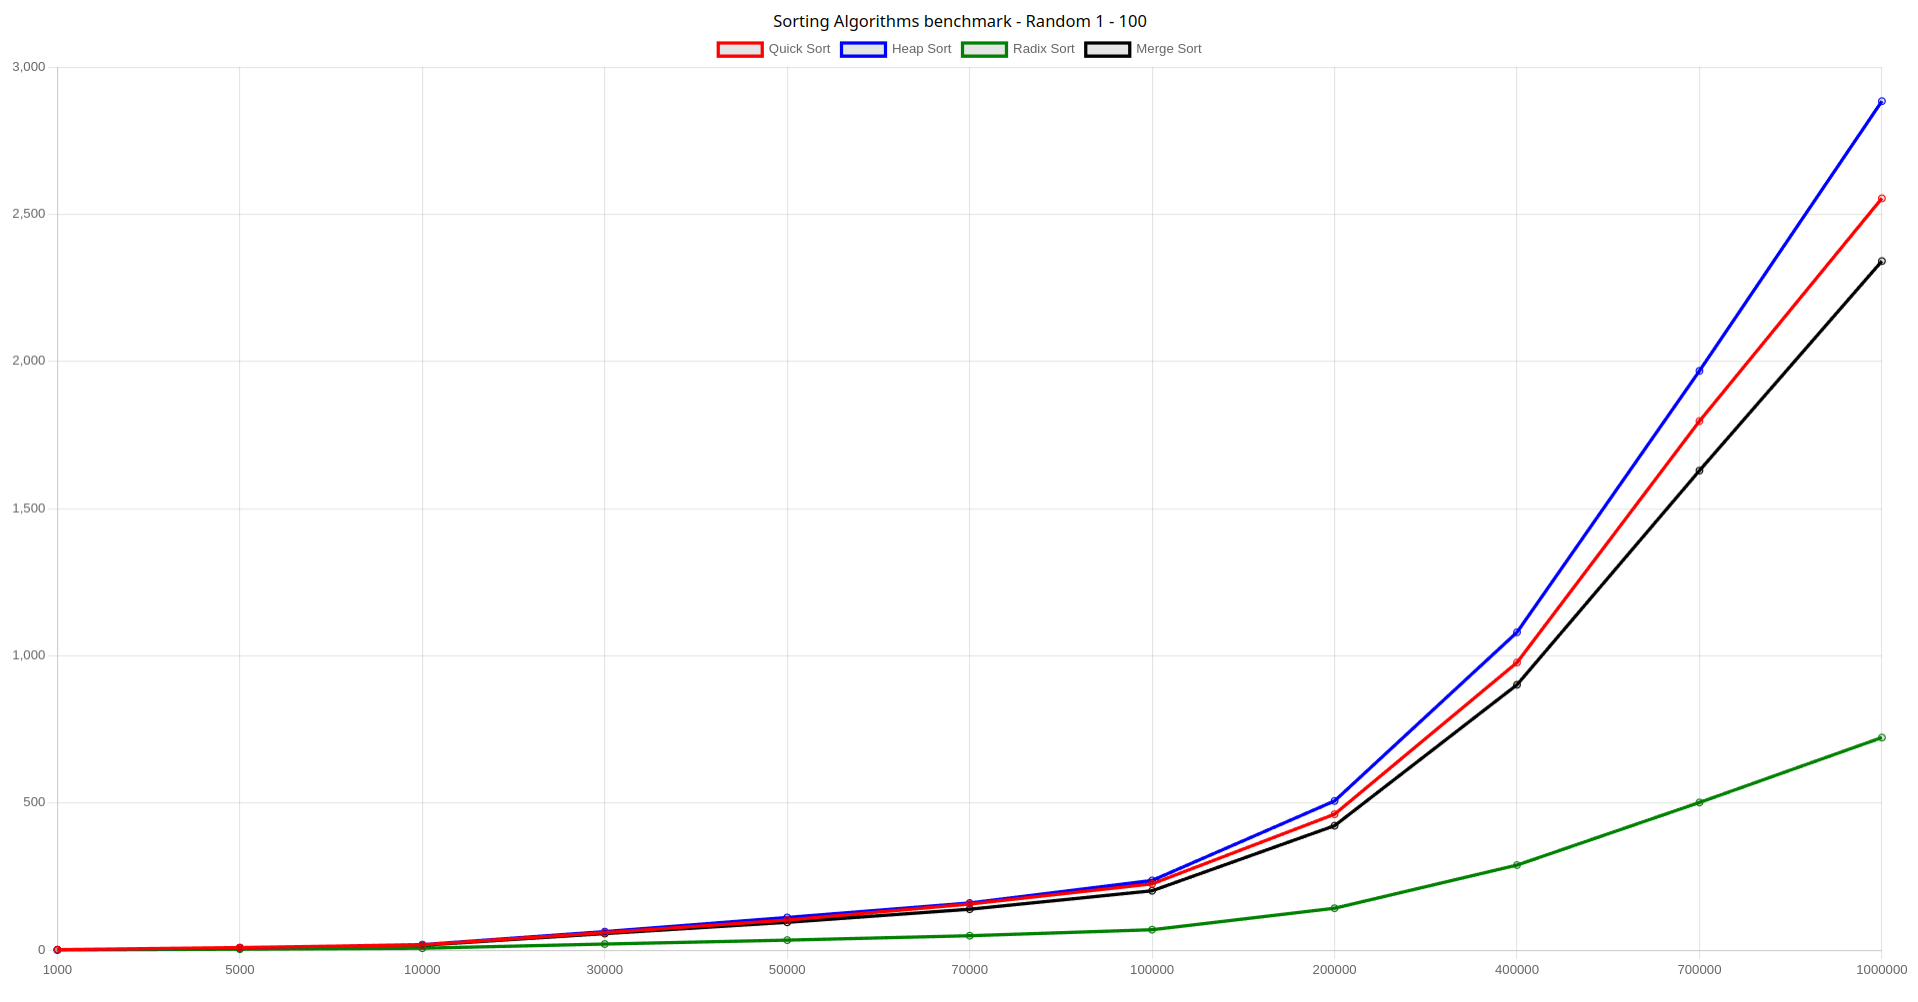
\includegraphics[width=1\textwidth]{random100.png}
    \caption{Random numbers from range 1 - 100}
    \label{fig:rand100}
\end{figure}

\begin{figure}[h]
    \centering
    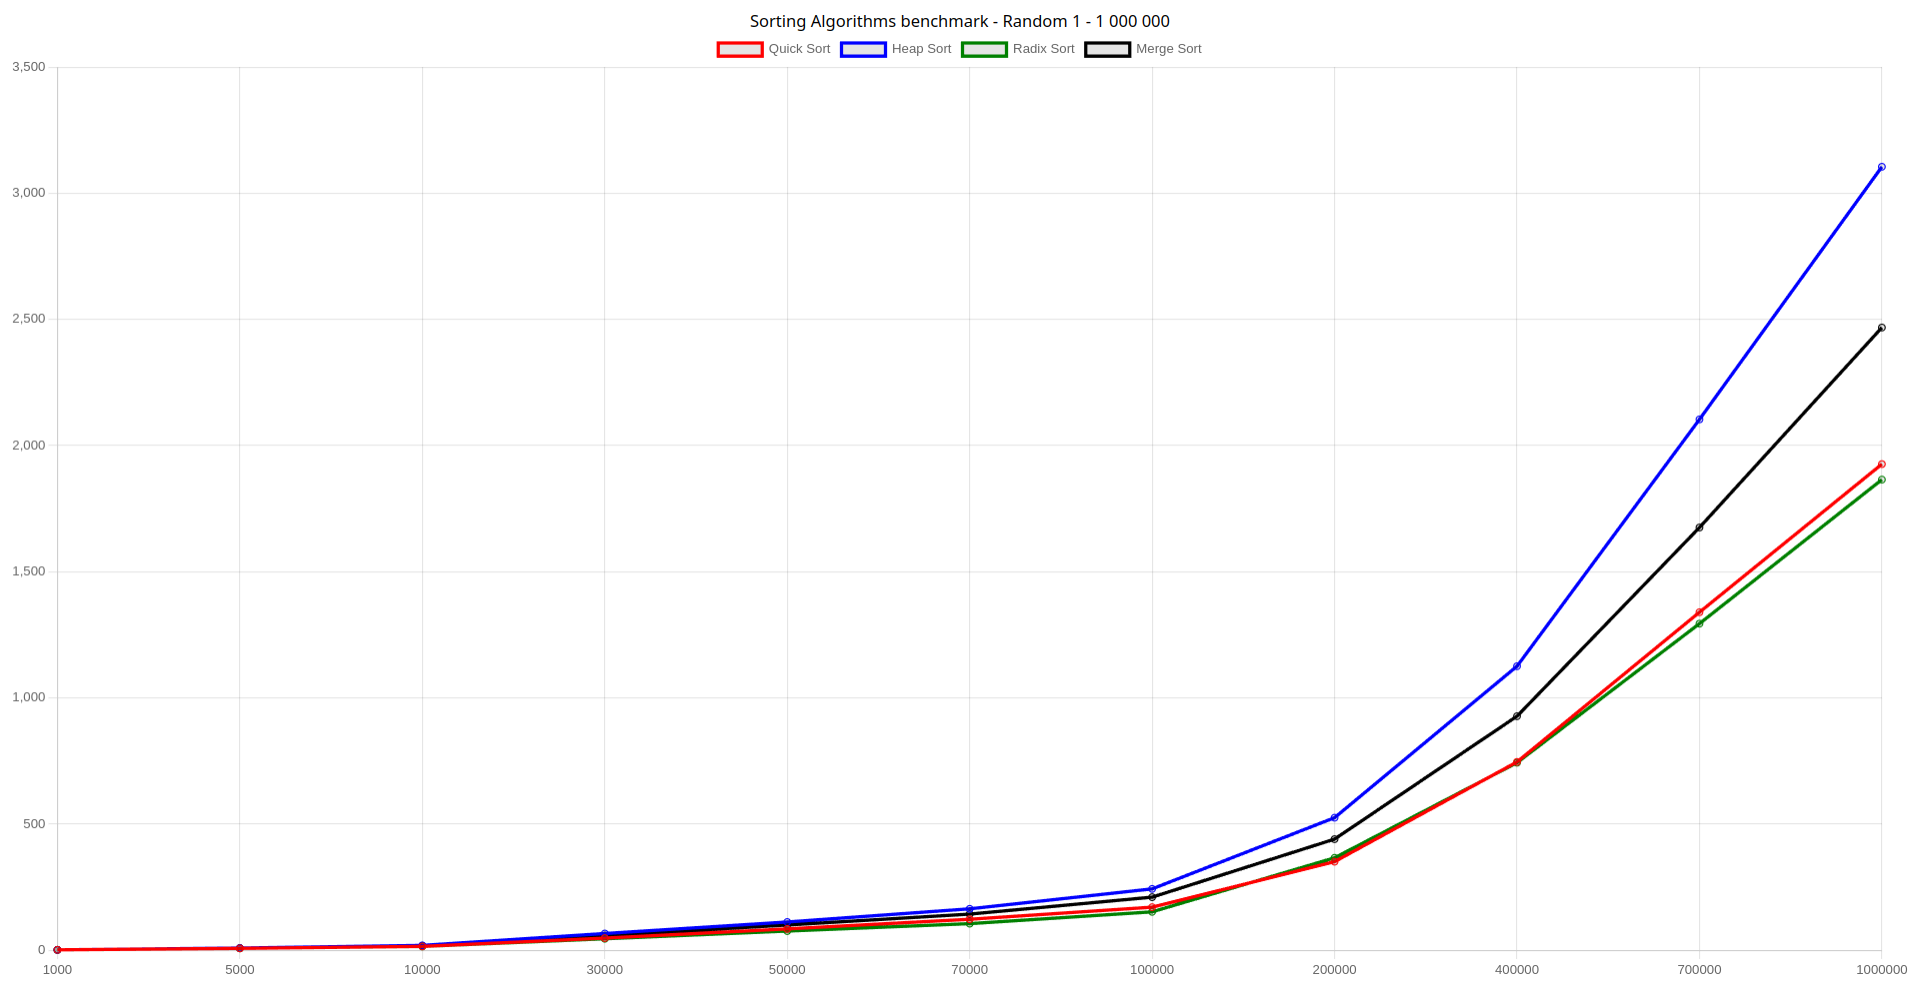
\includegraphics[width=1\textwidth]{random10^6.png}
    \caption{Random numbers from range 1 - 1 000 000}
    \label{fig:rand1000000}
\end{figure}

\begin{figure}[h]
    \centering
    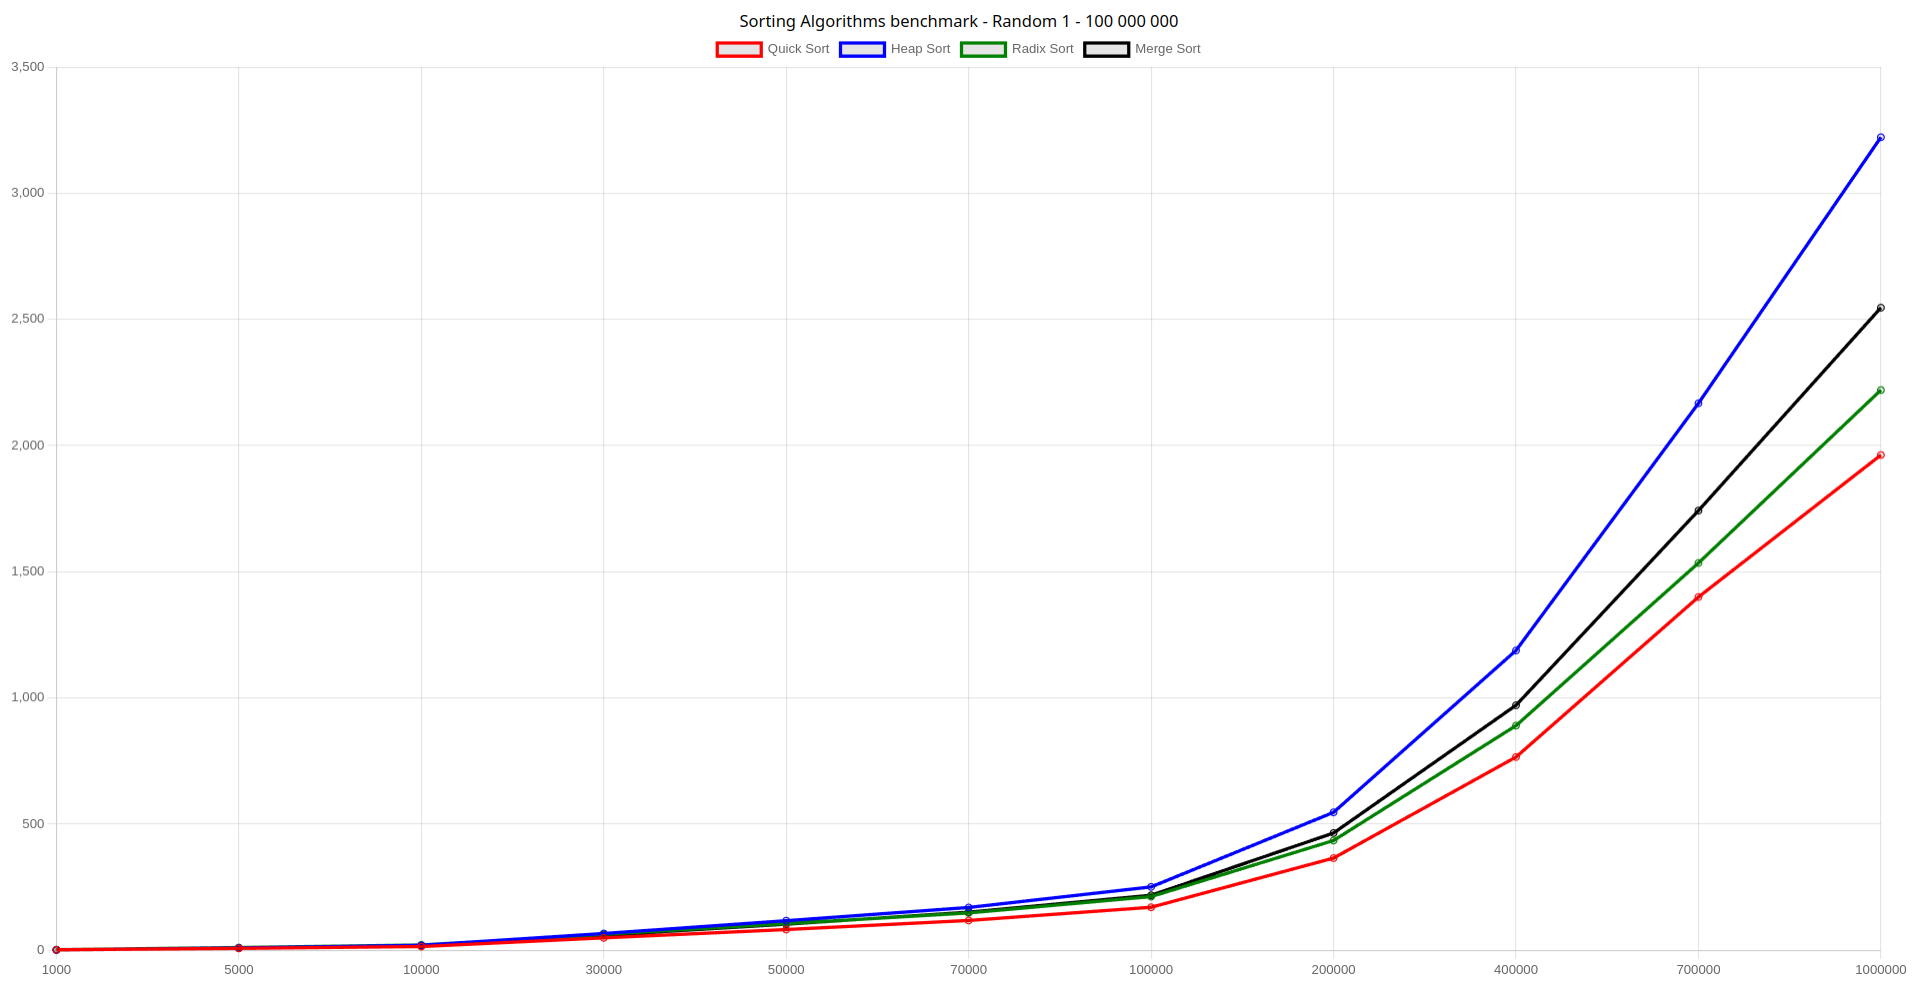
\includegraphics[width=1\textwidth]{random10^8.png}
    \caption{Random numbers from range 1 - 100 000 000}
    \label{fig:rand100000000}
\end{figure}

\clearpage
We can easily observe that even if sorting algorithms 
are performing nearly the same as expected, \textit{\textbf{Radix sort}} is vastly influenced 
by the number of digits implied in the input data. You can see the differences in
figure \ref{fig:rand100} and figure \ref{fig:rand100000000}. Even if the length of arrays is still the 
same, Radix sort has to perform editional placements of elements for each aditional digit that the
largest number has. This is why it is important to mention that even if performance of 
Radix sort can be low, it's time execution is highly influenced by the number of digits of the 
largest number and complexity of the Radix sort is always mentioned as \textit{\textbf{O(n*d)}}, not O(n)

\begin{figure}[h]
    \centering
    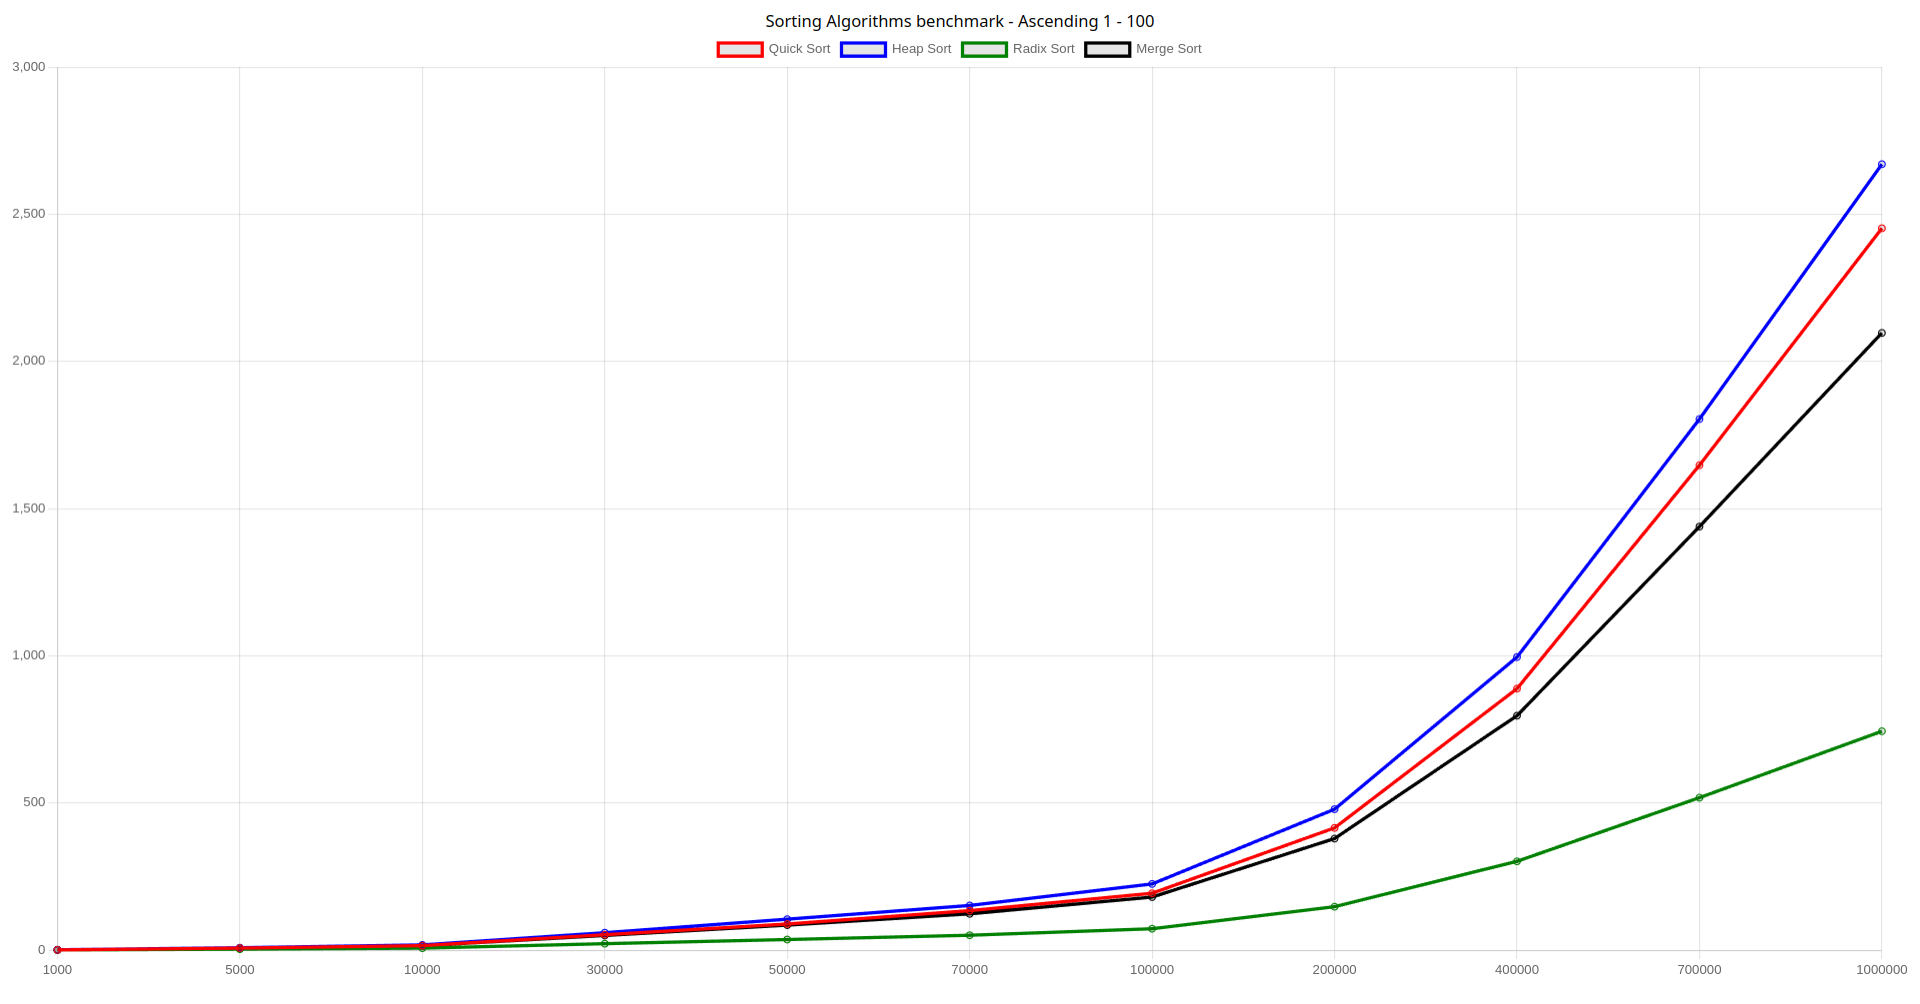
\includegraphics[width=1\textwidth]{ascen100.png}
    \caption{Numbers in ascending order in range 1 - 100}
    \label{fig:ascending100}
\end{figure}

\begin{figure}[h]
    \centering
    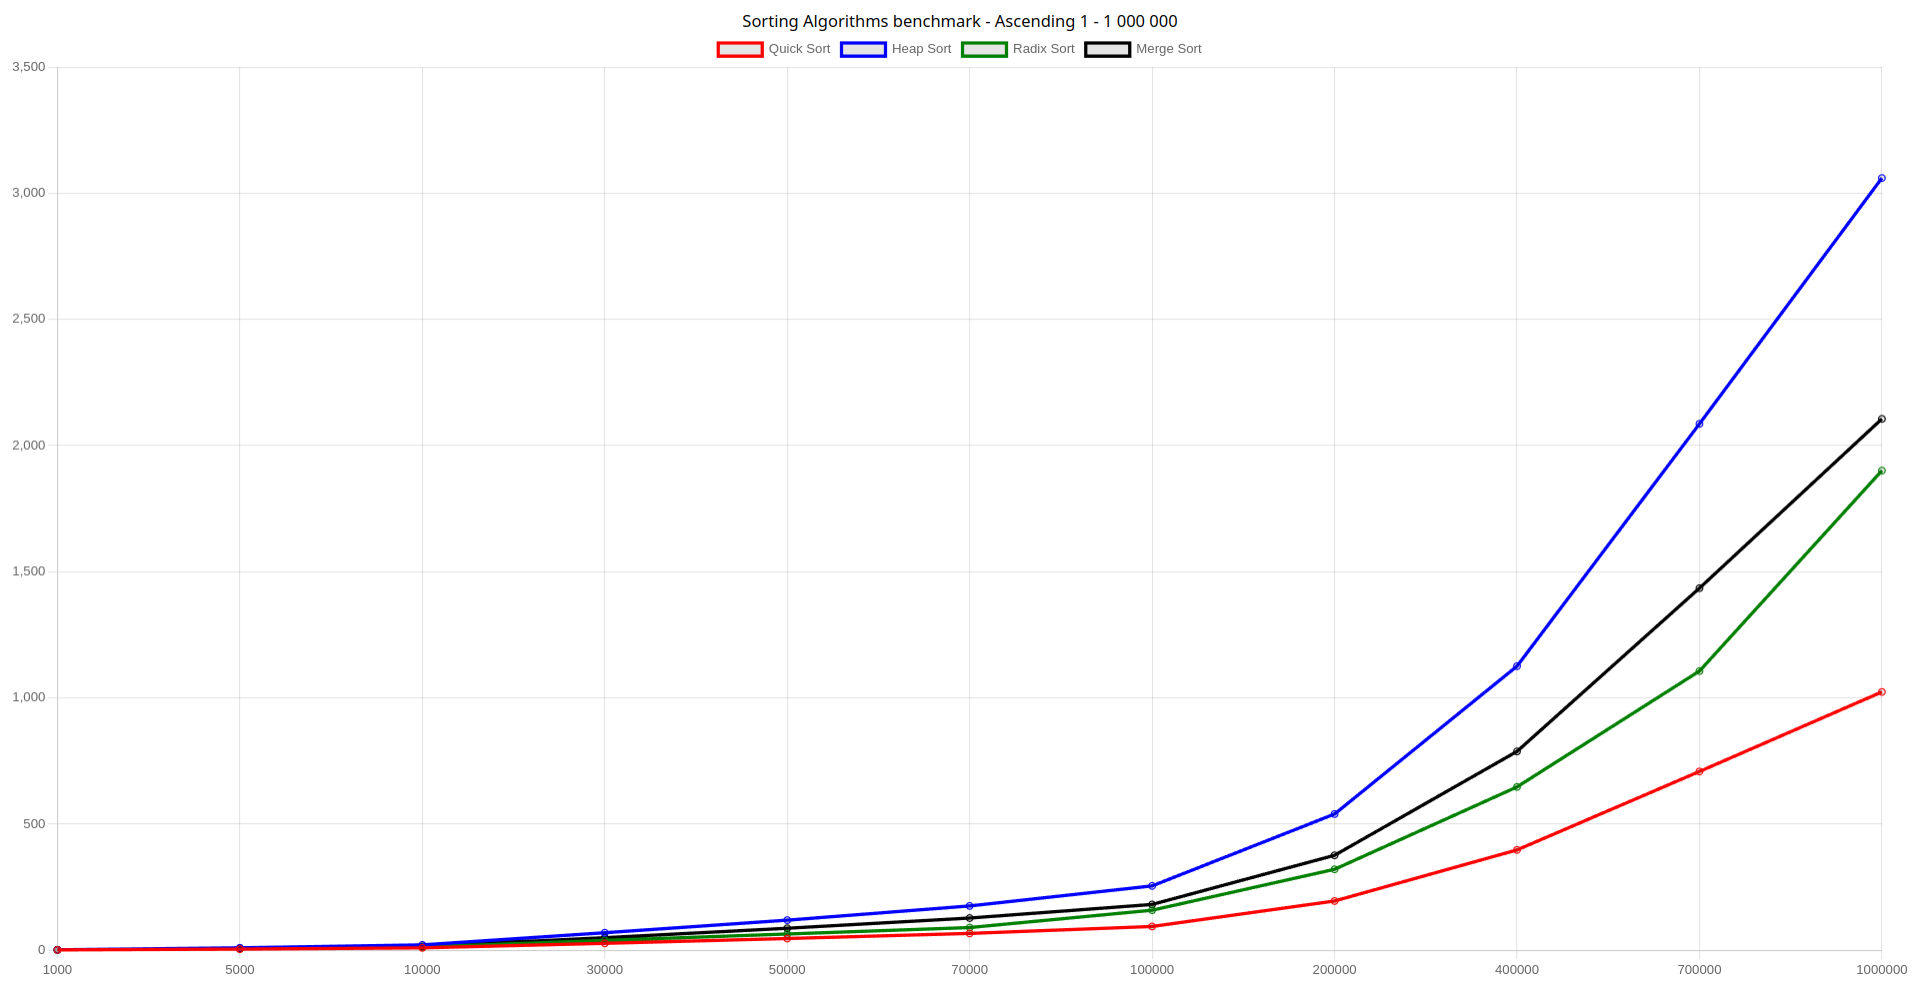
\includegraphics[width=1\textwidth]{ascen1000000.png}
    \caption{Numbers in ascending order in range 1 - 100 000 000}
    \label{fig:ascending1000000}
\end{figure}
\clearpage
Besides the slowdown of Radix sort already described above we can see that \textbf{Quick Sort} is already loosing
his positions to Merge Sort (figure \ref{fig:ascending1000000} and only there). This happens because of logic behind the Quick sort. To 
perform the sorting it uses a \textit{pivot}. It is a flag that is used to arrange the 
elements smaller than pivot to the left side of the partition 
and the greater numbers to the right side of the partition. 
In best case, the Time Complexity of Quick sort 
is \textbf{\textit{O(n*logN)}}. This scenario can occur if everytime the chosen pivot is the element that should
be placed in the middle of the partition. BUT. \textbf{If on each iteration the chosen pivot 
leads to biggest possible number of comparisons, then the Time Complexity 
of Quick Sort is \textit{$O(n^2)$}}. In this case smaller range meant a big number of redundant comparisons 
between same elements. This issue is not so evident in figure \ref{fig:ascending1000000}

It will perform the comparison on all the elements of the array with no proper partitioning, because elements are repeating themself. Same effect we can see on next diagrams.

Also we can see a speed improvement for other sorting algorithms.


\begin{figure}[h]
    \centering
    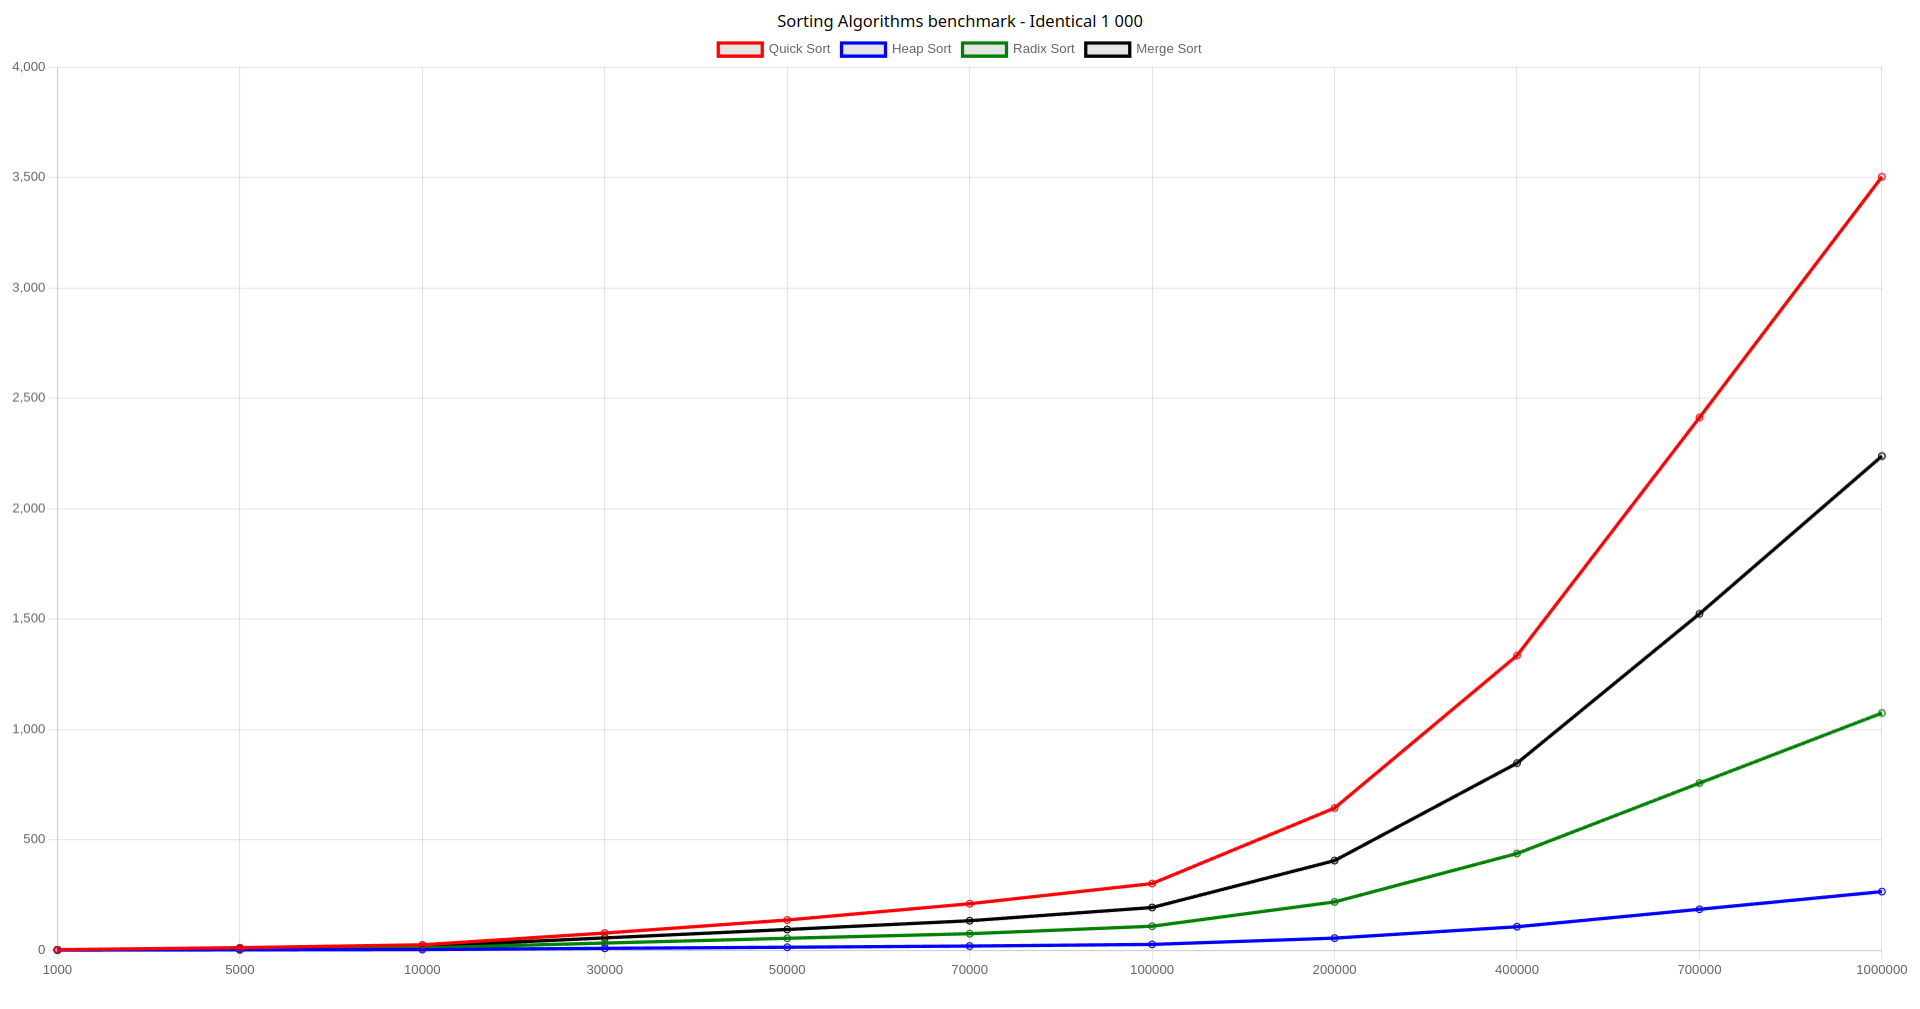
\includegraphics[width=1\textwidth]{iden1000.png}
    \caption{Array with the same number 1000}
    \label{fig:identical1000}
\end{figure}

\begin{figure}[h]
    \centering
    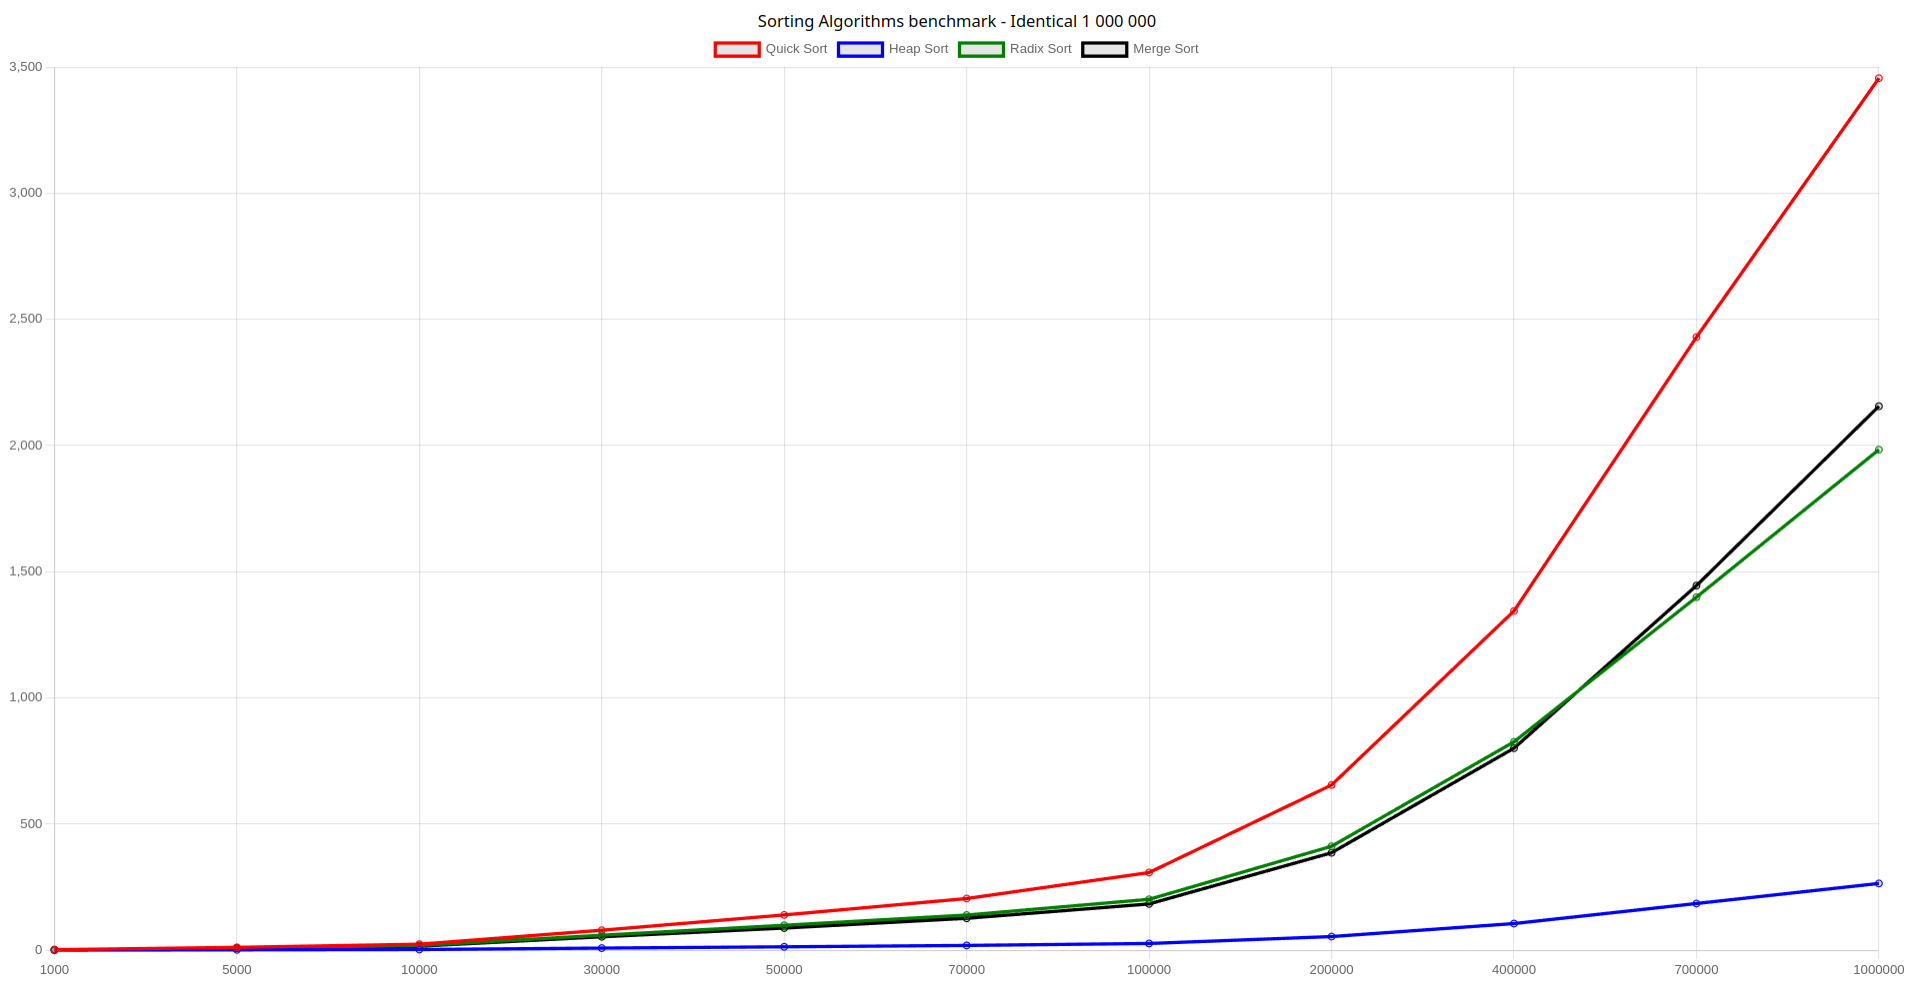
\includegraphics[width=1\textwidth]{iden1000000.png}
    \caption{Array with the same number 1 000 000}
    \label{fig:identical1000000}
\end{figure}

\clearpage
Identical numbers are drastically disadvantaging Quick sort, because it has to 
do the comparisons literarly for all of the elements in current partition and reach its highest 
time complexity. 

On the other hand Heap sort is the fastest in this case. This happens because the heapify function does not 
have to swap any of the elements in the heap and can directly return the same 
tree as the result. Only thing that it needs to do is to pass each node and just check it.


\clearpage
\section*{Graphical Representation}
\hspace{0.8cm}
Graphical representation was done in React, deployed on Vercel and can be accessed online by link \cite{site}.
I decided to provide a more practical representation of the sorting algorithms rather than moving bars on the
screen. In my subjective opinion bars are not a good way to understand sorting algorithms.
\begin{figure}[h]
    \centering
    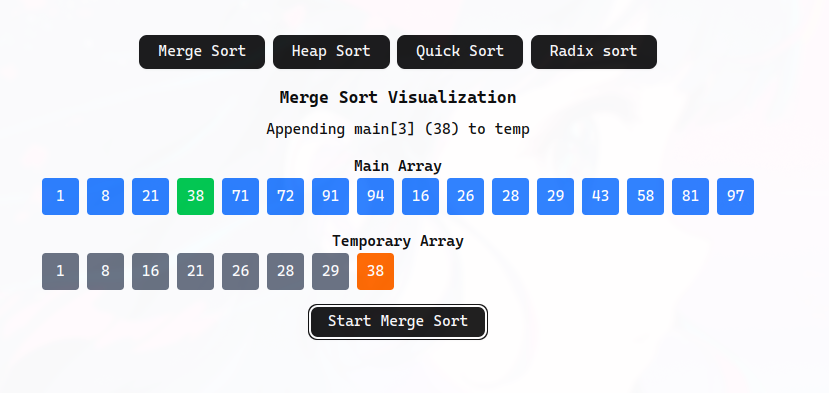
\includegraphics[width=0.9\textwidth]{merge_im.png}
    \caption{Representation of Merge Sort}
\end{figure}

\begin{figure}[h]
    \centering
    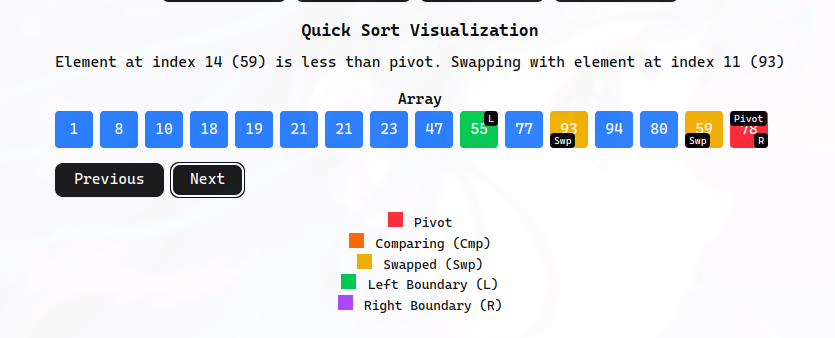
\includegraphics[width=0.9\textwidth]{quick_im.png}
    \caption{Representation of Quick Sort}
\end{figure}

\begin{figure}[h]
    \centering
    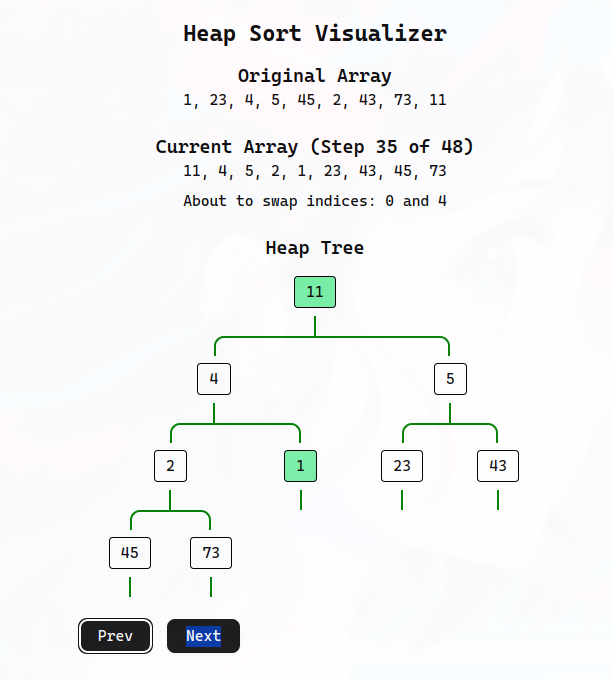
\includegraphics[width=0.7\textwidth]{heap_im.png}
    \caption{Representation of Heap Sort}
\end{figure}

\begin{figure}[h]
    \centering
    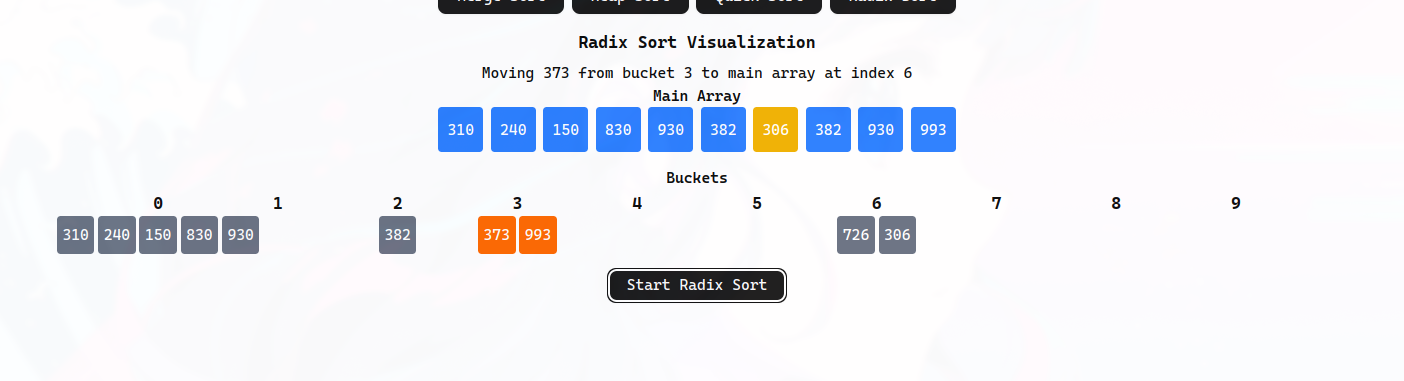
\includegraphics[width=1\textwidth]{radix_im.png}
    \caption{Representation of Radix Sort}
\end{figure}
\clearpage
\section*{Conclusions}
\hspace{0.6cm} 
In conclusion I can say that the most reliable and predictable sorting algorithm is Merging Sort.
In each case it performed relatively well, which is a very good result considering 
that Quick Sort(considered the fastest sorting algorithm) is running with 
complexity near to $n^2$ in some cases. If you look at each metric, you can see that the execution time of
Merge Sort is constant. This is why it is mostly used as default sorting algorithm.

\begin{thebibliography}{9}

  \bibitem{bytecoderef} \href{https://medium.com/dailyjs/understanding-v8s-bytecode-317d46c94775}{Franceska
      Hinkelman (2017) - Understanding bytecode \emph{Medium}}
  \bibitem{github} \href{https://github.com/DdimaPos/AA-labs/tree/main/Lab2}{GitHub repository of current laboratory work}
  \bibitem{site} \href{https://sorting-algorithms-visualizer-rho.vercel.app/}{Graphical representation of the sorting algorithms}
\end{thebibliography}
\end{document}
